% Options for packages loaded elsewhere
\PassOptionsToPackage{unicode}{hyperref}
\PassOptionsToPackage{hyphens}{url}
%
\documentclass[
]{article}
\usepackage{lmodern}
\usepackage{amsmath}
\usepackage{ifxetex,ifluatex}
\ifnum 0\ifxetex 1\fi\ifluatex 1\fi=0 % if pdftex
  \usepackage[T1]{fontenc}
  \usepackage[utf8]{inputenc}
  \usepackage{textcomp} % provide euro and other symbols
  \usepackage{amssymb}
\else % if luatex or xetex
  \usepackage{unicode-math}
  \defaultfontfeatures{Scale=MatchLowercase}
  \defaultfontfeatures[\rmfamily]{Ligatures=TeX,Scale=1}
\fi
% Use upquote if available, for straight quotes in verbatim environments
\IfFileExists{upquote.sty}{\usepackage{upquote}}{}
\IfFileExists{microtype.sty}{% use microtype if available
  \usepackage[]{microtype}
  \UseMicrotypeSet[protrusion]{basicmath} % disable protrusion for tt fonts
}{}
\makeatletter
\@ifundefined{KOMAClassName}{% if non-KOMA class
  \IfFileExists{parskip.sty}{%
    \usepackage{parskip}
  }{% else
    \setlength{\parindent}{0pt}
    \setlength{\parskip}{6pt plus 2pt minus 1pt}}
}{% if KOMA class
  \KOMAoptions{parskip=half}}
\makeatother
\usepackage{xcolor}
\IfFileExists{xurl.sty}{\usepackage{xurl}}{} % add URL line breaks if available
\IfFileExists{bookmark.sty}{\usepackage{bookmark}}{\usepackage{hyperref}}
\hypersetup{
  pdftitle={Gestion de Portefeuille},
  hidelinks,
  pdfcreator={LaTeX via pandoc}}
\urlstyle{same} % disable monospaced font for URLs
\usepackage[margin=1in]{geometry}
\usepackage{color}
\usepackage{fancyvrb}
\newcommand{\VerbBar}{|}
\newcommand{\VERB}{\Verb[commandchars=\\\{\}]}
\DefineVerbatimEnvironment{Highlighting}{Verbatim}{commandchars=\\\{\}}
% Add ',fontsize=\small' for more characters per line
\usepackage{framed}
\definecolor{shadecolor}{RGB}{248,248,248}
\newenvironment{Shaded}{\begin{snugshade}}{\end{snugshade}}
\newcommand{\AlertTok}[1]{\textcolor[rgb]{0.94,0.16,0.16}{#1}}
\newcommand{\AnnotationTok}[1]{\textcolor[rgb]{0.56,0.35,0.01}{\textbf{\textit{#1}}}}
\newcommand{\AttributeTok}[1]{\textcolor[rgb]{0.77,0.63,0.00}{#1}}
\newcommand{\BaseNTok}[1]{\textcolor[rgb]{0.00,0.00,0.81}{#1}}
\newcommand{\BuiltInTok}[1]{#1}
\newcommand{\CharTok}[1]{\textcolor[rgb]{0.31,0.60,0.02}{#1}}
\newcommand{\CommentTok}[1]{\textcolor[rgb]{0.56,0.35,0.01}{\textit{#1}}}
\newcommand{\CommentVarTok}[1]{\textcolor[rgb]{0.56,0.35,0.01}{\textbf{\textit{#1}}}}
\newcommand{\ConstantTok}[1]{\textcolor[rgb]{0.00,0.00,0.00}{#1}}
\newcommand{\ControlFlowTok}[1]{\textcolor[rgb]{0.13,0.29,0.53}{\textbf{#1}}}
\newcommand{\DataTypeTok}[1]{\textcolor[rgb]{0.13,0.29,0.53}{#1}}
\newcommand{\DecValTok}[1]{\textcolor[rgb]{0.00,0.00,0.81}{#1}}
\newcommand{\DocumentationTok}[1]{\textcolor[rgb]{0.56,0.35,0.01}{\textbf{\textit{#1}}}}
\newcommand{\ErrorTok}[1]{\textcolor[rgb]{0.64,0.00,0.00}{\textbf{#1}}}
\newcommand{\ExtensionTok}[1]{#1}
\newcommand{\FloatTok}[1]{\textcolor[rgb]{0.00,0.00,0.81}{#1}}
\newcommand{\FunctionTok}[1]{\textcolor[rgb]{0.00,0.00,0.00}{#1}}
\newcommand{\ImportTok}[1]{#1}
\newcommand{\InformationTok}[1]{\textcolor[rgb]{0.56,0.35,0.01}{\textbf{\textit{#1}}}}
\newcommand{\KeywordTok}[1]{\textcolor[rgb]{0.13,0.29,0.53}{\textbf{#1}}}
\newcommand{\NormalTok}[1]{#1}
\newcommand{\OperatorTok}[1]{\textcolor[rgb]{0.81,0.36,0.00}{\textbf{#1}}}
\newcommand{\OtherTok}[1]{\textcolor[rgb]{0.56,0.35,0.01}{#1}}
\newcommand{\PreprocessorTok}[1]{\textcolor[rgb]{0.56,0.35,0.01}{\textit{#1}}}
\newcommand{\RegionMarkerTok}[1]{#1}
\newcommand{\SpecialCharTok}[1]{\textcolor[rgb]{0.00,0.00,0.00}{#1}}
\newcommand{\SpecialStringTok}[1]{\textcolor[rgb]{0.31,0.60,0.02}{#1}}
\newcommand{\StringTok}[1]{\textcolor[rgb]{0.31,0.60,0.02}{#1}}
\newcommand{\VariableTok}[1]{\textcolor[rgb]{0.00,0.00,0.00}{#1}}
\newcommand{\VerbatimStringTok}[1]{\textcolor[rgb]{0.31,0.60,0.02}{#1}}
\newcommand{\WarningTok}[1]{\textcolor[rgb]{0.56,0.35,0.01}{\textbf{\textit{#1}}}}
\usepackage{graphicx}
\makeatletter
\def\maxwidth{\ifdim\Gin@nat@width>\linewidth\linewidth\else\Gin@nat@width\fi}
\def\maxheight{\ifdim\Gin@nat@height>\textheight\textheight\else\Gin@nat@height\fi}
\makeatother
% Scale images if necessary, so that they will not overflow the page
% margins by default, and it is still possible to overwrite the defaults
% using explicit options in \includegraphics[width, height, ...]{}
\setkeys{Gin}{width=\maxwidth,height=\maxheight,keepaspectratio}
% Set default figure placement to htbp
\makeatletter
\def\fps@figure{htbp}
\makeatother
\setlength{\emergencystretch}{3em} % prevent overfull lines
\providecommand{\tightlist}{%
  \setlength{\itemsep}{0pt}\setlength{\parskip}{0pt}}
\setcounter{secnumdepth}{-\maxdimen} % remove section numbering
\usepackage[utf8]{inputenc}
\usepackage{amsmath}
\usepackage{amsfonts}
\usepackage{amssymb}
\usepackage{booktabs}
\usepackage{longtable}
\usepackage{array}
\usepackage{multirow}
\usepackage{wrapfig}
\usepackage{float}
\usepackage{colortbl}
\usepackage{pdflscape}
\usepackage{tabu}
\usepackage{threeparttable}
\usepackage{threeparttablex}
\usepackage[normalem]{ulem}
\usepackage{makecell}
\usepackage{xcolor}
\ifluatex
  \usepackage{selnolig}  % disable illegal ligatures
\fi

\title{Gestion de Portefeuille}
\usepackage{etoolbox}
\makeatletter
\providecommand{\subtitle}[1]{% add subtitle to \maketitle
  \apptocmd{\@title}{\par {\large #1 \par}}{}{}
}
\makeatother
\subtitle{TP-1: Analyse de l'indice CAC40}
\author{}
\date{\vspace{-2.5em}Version: 15 fév 2022}

\begin{document}
\maketitle

\begin{Shaded}
\begin{Highlighting}[]
\FunctionTok{library}\NormalTok{(lubridate)}
\FunctionTok{library}\NormalTok{(Hmisc)}
\FunctionTok{library}\NormalTok{(tseries)}
\FunctionTok{library}\NormalTok{(timeSeries)}
\FunctionTok{library}\NormalTok{(kableExtra)}


\NormalTok{get.src.folder }\OtherTok{\textless{}{-}} \ControlFlowTok{function}\NormalTok{() \{}
  \FunctionTok{path.expand}\NormalTok{(}\StringTok{"../GP/src"}\NormalTok{)}
\NormalTok{\}}

\NormalTok{get.data.folder }\OtherTok{\textless{}{-}} \ControlFlowTok{function}\NormalTok{() \{}
  \FunctionTok{path.expand}\NormalTok{(}\StringTok{"../GP/data"}\NormalTok{)}
\NormalTok{\}}

\FunctionTok{source}\NormalTok{(}\FunctionTok{file.path}\NormalTok{(}\FunctionTok{get.src.folder}\NormalTok{(), }\StringTok{\textquotesingle{}utils.R\textquotesingle{}}\NormalTok{))}
\end{Highlighting}
\end{Shaded}

\begin{verbatim}
## Warning: package 'spam' was built under R version 4.0.5
\end{verbatim}

\begin{Shaded}
\begin{Highlighting}[]
\FunctionTok{source}\NormalTok{(}\FunctionTok{file.path}\NormalTok{(}\FunctionTok{get.src.folder}\NormalTok{(), }\StringTok{\textquotesingle{}FileUtils.R\textquotesingle{}}\NormalTok{))}
\end{Highlighting}
\end{Shaded}

\hypertarget{les-donnuxe9es}{%
\subsection{Les données}\label{les-donnuxe9es}}

On charge les séries de rendements pour l'indice et les composants de
l'indice.

\begin{Shaded}
\begin{Highlighting}[]
\NormalTok{  ts.all }\OtherTok{\textless{}{-}} \FunctionTok{get.all.ts}\NormalTok{(}\StringTok{\textquotesingle{}CAC40\textquotesingle{}}\NormalTok{, }\AttributeTok{tickers=}\ConstantTok{NULL}\NormalTok{, }\AttributeTok{returns =} \ConstantTok{TRUE}\NormalTok{,}
    \AttributeTok{dt.start =} \FunctionTok{dmy}\NormalTok{(}\StringTok{\textquotesingle{}01Jul2007\textquotesingle{}}\NormalTok{), }\AttributeTok{combine =}\NormalTok{ T)}
  
  \CommentTok{\# bad data for Valeo}
\NormalTok{  ts.all }\OtherTok{\textless{}{-}}\NormalTok{ ts.all[,}\SpecialCharTok{{-}}\DecValTok{17}\NormalTok{]}
  
  \CommentTok{\# keep good data window}
\NormalTok{  ts.all }\OtherTok{\textless{}{-}} \FunctionTok{window}\NormalTok{(ts.all, }\FunctionTok{dmy}\NormalTok{(}\StringTok{\textquotesingle{}01Jul2007\textquotesingle{}}\NormalTok{), }
                   \FunctionTok{dmy}\NormalTok{(}\StringTok{\textquotesingle{}01Jan2009\textquotesingle{}}\NormalTok{))}
  
  \CommentTok{\# merge with cac40 index}
\NormalTok{  cac.index }\OtherTok{\textless{}{-}} \FunctionTok{get.ts}\NormalTok{(}\StringTok{\textquotesingle{}fchi\textquotesingle{}}\NormalTok{, }\StringTok{\textquotesingle{}CAC40\textquotesingle{}}\NormalTok{)}

\NormalTok{  cac.ret }\OtherTok{\textless{}{-}} \FunctionTok{returns}\NormalTok{(cac.index)}
  \FunctionTok{names}\NormalTok{(cac.ret) }\OtherTok{\textless{}{-}} \StringTok{\textquotesingle{}CAC40\textquotesingle{}}
\NormalTok{  ts.all }\OtherTok{\textless{}{-}} \FunctionTok{removeNA}\NormalTok{(}\FunctionTok{cbind}\NormalTok{(ts.all, cac.ret))}
\end{Highlighting}
\end{Shaded}

\begin{Shaded}
\begin{Highlighting}[]
\FunctionTok{plot}\NormalTok{(ts.all[, }\FunctionTok{c}\NormalTok{(}\DecValTok{1}\NormalTok{,}\DecValTok{2}\NormalTok{,}\DecValTok{3}\NormalTok{)], }\AttributeTok{main=}\StringTok{\textquotesingle{}Rendement quotidien\textquotesingle{}}\NormalTok{)}
\end{Highlighting}
\end{Shaded}

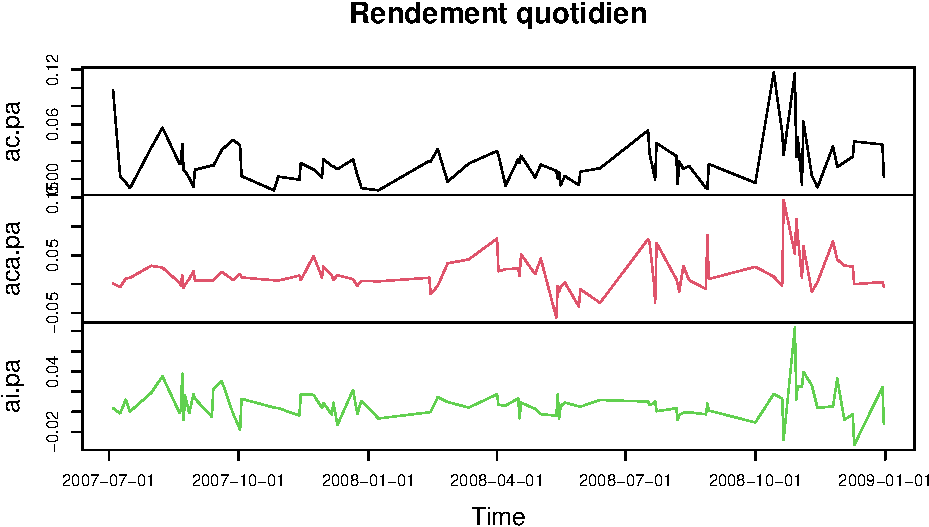
\includegraphics{TP1_files/figure-latex/plot-cac-1-1.pdf}

Puis on filtre les points suspects: rendements supérieur à 8 s.d.

\begin{Shaded}
\begin{Highlighting}[]
  \CommentTok{\# flag bad data points: \textgreater{} * \textbackslash{}sigma}
\NormalTok{  good.limit }\OtherTok{\textless{}{-}} \DecValTok{8}\SpecialCharTok{*}\FunctionTok{apply}\NormalTok{(ts.all, }\DecValTok{2}\NormalTok{, sd)}
  
\NormalTok{  ts.bad }\OtherTok{\textless{}{-}}\NormalTok{ ts.all}\SpecialCharTok{*}\ConstantTok{FALSE}
  \ControlFlowTok{for}\NormalTok{(j }\ControlFlowTok{in} \FunctionTok{seq}\NormalTok{(}\FunctionTok{ncol}\NormalTok{(ts.bad))) \{}
\NormalTok{    ts.bad[,j] }\OtherTok{\textless{}{-}} \FunctionTok{abs}\NormalTok{(ts.all[,j]) }\SpecialCharTok{\textgreater{}}\NormalTok{ good.limit[j]}
\NormalTok{  \}}
\NormalTok{  good.index }\OtherTok{\textless{}{-}} \SpecialCharTok{!}\FunctionTok{apply}\NormalTok{(ts.bad,}\DecValTok{1}\NormalTok{,any)}
\NormalTok{  ts.all }\OtherTok{\textless{}{-}}\NormalTok{ ts.all[good.index,]}
\end{Highlighting}
\end{Shaded}

Finalement, on calcule les rendements hebdomadaires:

\begin{Shaded}
\begin{Highlighting}[]
  \CommentTok{\# aggregate returns by week}
\NormalTok{  by }\OtherTok{\textless{}{-}} \FunctionTok{timeSequence}\NormalTok{(}\AttributeTok{from=}\FunctionTok{start}\NormalTok{(ts.all), }
                     \AttributeTok{to=}\FunctionTok{end}\NormalTok{(ts.all), }\AttributeTok{by=}\StringTok{\textquotesingle{}week\textquotesingle{}}\NormalTok{)}
\NormalTok{  ts.all.weekly }\OtherTok{\textless{}{-}} \FunctionTok{aggregate}\NormalTok{(ts.all, by, sum)}

\NormalTok{  ts.stocks }\OtherTok{\textless{}{-}}\NormalTok{ ts.all.weekly[,}\SpecialCharTok{{-}}\DecValTok{40}\NormalTok{]}
\NormalTok{  ts.index }\OtherTok{\textless{}{-}}\NormalTok{ ts.all.weekly[,}\DecValTok{40}\NormalTok{]}
\end{Highlighting}
\end{Shaded}

\begin{Shaded}
\begin{Highlighting}[]
\FunctionTok{plot}\NormalTok{(ts.index, }\AttributeTok{main=}\StringTok{\textquotesingle{}Rendement hebdomadaire de l}\SpecialCharTok{\textbackslash{}\textquotesingle{}}\StringTok{indice CAC40\textquotesingle{}}\NormalTok{)}
\end{Highlighting}
\end{Shaded}

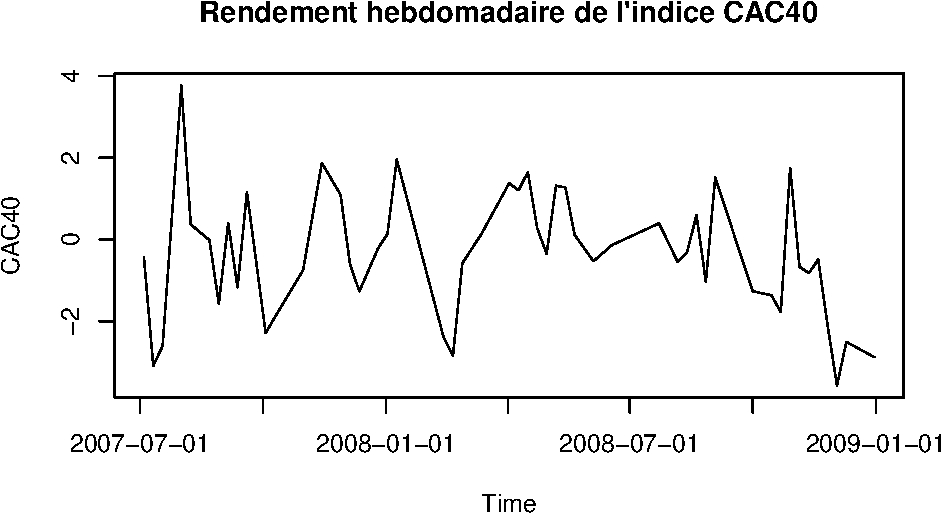
\includegraphics{TP1_files/figure-latex/plot-cac-2-1.pdf}

\hypertarget{calcul-de-correlation}{%
\subsection{Calcul de correlation}\label{calcul-de-correlation}}

\begin{itemize}
\item
  Calculer la matrice de corrélation des actions de l'indice.
\item
  Rechercher des actions fortement corrélées et d'autres qui semblent
  indépendantes. Justifier ces observations en considérant la nature des
  entreprises.
\item
  Choisir 3 titres, et reproduire la figure 3.5, page 35 du manuel de B.
  Pfaff. Commenter les résultats obtenus.
\end{itemize}

\hypertarget{analyse-en-composantes-principales}{%
\subsection{Analyse en composantes
principales}\label{analyse-en-composantes-principales}}

\begin{itemize}
\tightlist
\item
  Effectuer une ACP de la matrice de covariance des rendements
  hebdomadaires
\item
  Observer les projections des variables sur les premiers vecteurs
  propres, et tenter de fournir une interprétation économique de vos
  observations.
\end{itemize}

\hypertarget{calcul-de-correlation-1}{%
\subsection{Calcul de correlation}\label{calcul-de-correlation-1}}

\begin{Shaded}
\begin{Highlighting}[]
\NormalTok{cov.all }\OtherTok{\textless{}{-}} \FunctionTok{cor}\NormalTok{(ts.all)}
\NormalTok{cov.all[}\FunctionTok{lower.tri}\NormalTok{(cov.all)] }\OtherTok{\textless{}{-}} \ConstantTok{NA}
\FunctionTok{options}\NormalTok{(}\AttributeTok{knitr.kable.NA =} \StringTok{\textquotesingle{}\textquotesingle{}}\NormalTok{)}
\FunctionTok{kable}\NormalTok{(cov.all, }\StringTok{"latex"}\NormalTok{, }\AttributeTok{booktabs=}\NormalTok{T, }\AttributeTok{digits=}\DecValTok{2}\NormalTok{, }\AttributeTok{caption=}\StringTok{"Corrélation des rendements"}\NormalTok{) }\SpecialCharTok{\%\textgreater{}\%}
\FunctionTok{kable\_styling}\NormalTok{(}\AttributeTok{latex\_options=}\StringTok{"scale\_down"}\NormalTok{)}
\end{Highlighting}
\end{Shaded}

\begin{table}

\caption{\label{tab:correlation}Corrélation des rendements}
\centering
\resizebox{\linewidth}{!}{
\begin{tabular}[t]{lrrrrrrrrrrrrrrrrrrrrrrrrrrrrrrrrrrrrrrrr}
\toprule
  & ac.pa & aca.pa & ai.pa & air.pa & alo.pa & alu.pa & bn.pa & bnp.pa & ca.pa & cap.pa & cs.pa & dg.pa & edf.pa & ei.pa & en.pa & fp.pa & gle.pa & gsz.pa & ker.pa & lg.pa & lr.pa & mc.pa & ml.pa & mt.pa & or.pa & ora.pa & pub.pa & ri.pa & rno.pa & saf.pa & san.pa & sgo.pa & solb.br & su.pa & tec.pa & ug.pa & ul.pa & vie.pa & viv.pa & CAC40\\
\midrule
ac.pa & 1 & 0.29 & 0.40 & 0.27 & 0.36 & 0.40 & 0.20 & 0.28 & 0.38 & 0.39 & 0.52 & 0.55 & 0.38 & 0.10 & 0.40 & 0.51 & 0.49 & 0.27 & 0.57 & 0.38 & 0.44 & 0.26 & 0.35 & 0.16 & 0.10 & 0.32 & 0.33 & 0.45 & 0.51 & 0.20 & 0.25 & 0.62 & 0.28 & 0.50 & 0.29 & 0.47 & 0.46 & 0.03 & 0.13 & 0.18\\
aca.pa &  & 1.00 & 0.13 & 0.19 & 0.17 & 0.35 & -0.02 & 0.65 & -0.04 & 0.11 & 0.41 & 0.22 & 0.05 & -0.06 & 0.26 & 0.01 & 0.78 & 0.01 & 0.43 & 0.34 & 0.38 & 0.35 & 0.32 & 0.05 & -0.01 & 0.05 & 0.34 & 0.23 & 0.30 & 0.14 & 0.05 & 0.39 & 0.29 & 0.24 & 0.09 & 0.24 & 0.26 & 0.13 & 0.00 & 0.24\\
ai.pa &  &  & 1.00 & 0.22 & 0.53 & 0.19 & 0.35 & 0.20 & 0.29 & 0.23 & 0.54 & 0.55 & 0.42 & 0.24 & 0.43 & 0.60 & 0.17 & 0.36 & 0.36 & 0.21 & 0.29 & 0.33 & 0.41 & 0.54 & 0.27 & 0.44 & 0.29 & 0.22 & 0.38 & 0.20 & 0.34 & 0.48 & 0.42 & 0.49 & 0.27 & 0.24 & 0.40 & 0.17 & 0.46 & 0.34\\
air.pa &  &  &  & 1.00 & 0.09 & 0.29 & 0.26 & 0.34 & 0.33 & 0.33 & 0.38 & 0.37 & 0.29 & 0.10 & 0.45 & 0.21 & 0.18 & 0.24 & 0.25 & 0.00 & 0.32 & 0.34 & 0.16 & 0.03 & 0.26 & 0.31 & 0.20 & 0.23 & 0.33 & 0.44 & 0.27 & 0.38 & 0.29 & 0.35 & -0.06 & 0.24 & 0.19 & 0.12 & 0.37 & 0.33\\
alo.pa &  &  &  &  & 1.00 & 0.30 & 0.09 & 0.21 & 0.11 & 0.34 & 0.43 & 0.59 & 0.36 & 0.07 & 0.31 & 0.52 & 0.34 & 0.11 & 0.47 & 0.45 & 0.43 & 0.37 & 0.50 & 0.66 & 0.28 & 0.18 & 0.34 & 0.30 & 0.56 & 0.21 & -0.01 & 0.60 & 0.33 & 0.65 & 0.27 & 0.45 & 0.16 & 0.22 & 0.08 & 0.20\\
\addlinespace
alu.pa &  &  &  &  &  & 1.00 & -0.04 & 0.28 & 0.11 & 0.47 & 0.54 & 0.36 & 0.13 & 0.15 & 0.25 & 0.17 & 0.51 & 0.08 & 0.55 & 0.28 & 0.29 & 0.43 & 0.34 & 0.19 & 0.19 & 0.13 & 0.42 & 0.52 & 0.45 & 0.33 & 0.02 & 0.50 & 0.16 & 0.28 & 0.11 & 0.40 & 0.25 & -0.08 & 0.14 & 0.07\\
bn.pa &  &  &  &  &  &  & 1.00 & 0.02 & 0.44 & 0.15 & 0.17 & 0.30 & 0.20 & 0.10 & 0.26 & 0.34 & -0.09 & 0.37 & 0.08 & -0.01 & 0.13 & 0.18 & 0.13 & 0.04 & 0.38 & 0.36 & 0.10 & 0.10 & 0.10 & -0.01 & 0.50 & 0.17 & 0.22 & 0.20 & -0.02 & 0.03 & 0.23 & -0.15 & 0.36 & 0.32\\
bnp.pa &  &  &  &  &  &  &  & 1.00 & 0.00 & 0.20 & 0.43 & 0.31 & 0.09 & -0.08 & 0.48 & 0.14 & 0.64 & 0.14 & 0.37 & 0.16 & 0.30 & 0.39 & 0.33 & 0.19 & 0.21 & 0.13 & 0.31 & 0.03 & 0.47 & 0.19 & 0.12 & 0.47 & 0.41 & 0.29 & -0.04 & 0.27 & 0.12 & 0.29 & 0.10 & 0.33\\
ca.pa &  &  &  &  &  &  &  &  & 1.00 & 0.15 & 0.27 & 0.43 & 0.28 & 0.07 & 0.21 & 0.34 & 0.00 & 0.13 & 0.41 & 0.17 & 0.19 & 0.24 & 0.24 & -0.06 & 0.28 & 0.37 & 0.20 & 0.43 & 0.26 & 0.20 & 0.37 & 0.37 & 0.17 & 0.28 & 0.04 & 0.11 & 0.37 & -0.27 & 0.37 & 0.10\\
cap.pa &  &  &  &  &  &  &  &  &  & 1.00 & 0.37 & 0.40 & 0.25 & 0.12 & 0.28 & 0.22 & 0.24 & 0.29 & 0.43 & 0.27 & 0.35 & 0.44 & 0.28 & 0.25 & 0.14 & 0.11 & 0.26 & 0.27 & 0.28 & 0.37 & 0.06 & 0.46 & 0.27 & 0.34 & 0.15 & 0.25 & 0.20 & -0.06 & 0.28 & 0.14\\
\addlinespace
cs.pa &  &  &  &  &  &  &  &  &  &  & 1.00 & 0.49 & 0.31 & 0.22 & 0.36 & 0.38 & 0.56 & 0.27 & 0.64 & 0.21 & 0.32 & 0.49 & 0.45 & 0.20 & 0.29 & 0.44 & 0.43 & 0.44 & 0.61 & 0.34 & 0.27 & 0.63 & 0.26 & 0.52 & 0.20 & 0.34 & 0.35 & 0.20 & 0.31 & 0.26\\
dg.pa &  &  &  &  &  &  &  &  &  &  &  & 1.00 & 0.47 & 0.10 & 0.64 & 0.66 & 0.30 & 0.33 & 0.49 & 0.42 & 0.42 & 0.24 & 0.39 & 0.41 & 0.27 & 0.38 & 0.25 & 0.39 & 0.56 & 0.31 & 0.34 & 0.65 & 0.44 & 0.65 & 0.36 & 0.39 & 0.26 & 0.00 & 0.30 & 0.24\\
edf.pa &  &  &  &  &  &  &  &  &  &  &  &  & 1.00 & 0.18 & 0.45 & 0.59 & 0.13 & 0.43 & 0.30 & 0.18 & 0.32 & 0.18 & 0.20 & 0.30 & 0.12 & 0.27 & 0.06 & 0.26 & 0.31 & 0.26 & 0.26 & 0.46 & 0.20 & 0.38 & 0.27 & 0.27 & 0.13 & -0.01 & 0.12 & 0.18\\
ei.pa &  &  &  &  &  &  &  &  &  &  &  &  &  & 1.00 & 0.17 & 0.13 & -0.10 & 0.17 & 0.17 & 0.07 & -0.03 & 0.13 & 0.02 & 0.00 & 0.21 & 0.29 & -0.05 & 0.05 & 0.10 & 0.11 & 0.40 & 0.09 & -0.10 & 0.07 & -0.05 & 0.00 & 0.05 & -0.18 & 0.16 & 0.19\\
en.pa &  &  &  &  &  &  &  &  &  &  &  &  &  &  & 1.00 & 0.52 & 0.30 & 0.35 & 0.40 & 0.32 & 0.23 & 0.26 & 0.33 & 0.28 & 0.24 & 0.31 & 0.16 & 0.12 & 0.51 & 0.34 & 0.33 & 0.52 & 0.39 & 0.40 & 0.18 & 0.41 & 0.22 & 0.07 & 0.24 & 0.38\\
\addlinespace
fp.pa &  &  &  &  &  &  &  &  &  &  &  &  &  &  &  & 1.00 & 0.17 & 0.50 & 0.39 & 0.27 & 0.26 & 0.13 & 0.25 & 0.42 & 0.20 & 0.37 & 0.06 & 0.24 & 0.45 & 0.15 & 0.43 & 0.59 & 0.24 & 0.65 & 0.33 & 0.32 & 0.13 & -0.05 & 0.25 & 0.25\\
gle.pa &  &  &  &  &  &  &  &  &  &  &  &  &  &  &  &  & 1.00 & 0.01 & 0.55 & 0.37 & 0.38 & 0.37 & 0.39 & 0.22 & -0.01 & 0.07 & 0.38 & 0.32 & 0.55 & 0.16 & -0.03 & 0.52 & 0.22 & 0.36 & 0.21 & 0.44 & 0.27 & 0.31 & -0.04 & 0.23\\
gsz.pa &  &  &  &  &  &  &  &  &  &  &  &  &  &  &  &  &  & 1.00 & 0.17 & 0.01 & 0.23 & 0.19 & 0.09 & 0.18 & 0.21 & 0.35 & 0.00 & -0.16 & 0.17 & 0.03 & 0.31 & 0.24 & 0.22 & 0.20 & 0.16 & 0.18 & 0.09 & -0.28 & 0.29 & 0.37\\
ker.pa &  &  &  &  &  &  &  &  &  &  &  &  &  &  &  &  &  &  & 1.00 & 0.41 & 0.50 & 0.58 & 0.62 & 0.21 & 0.17 & 0.26 & 0.48 & 0.43 & 0.60 & 0.27 & 0.20 & 0.70 & 0.30 & 0.53 & 0.16 & 0.46 & 0.33 & 0.01 & 0.20 & 0.24\\
lg.pa &  &  &  &  &  &  &  &  &  &  &  &  &  &  &  &  &  &  &  & 1.00 & 0.33 & 0.22 & 0.38 & 0.33 & 0.03 & 0.02 & 0.39 & 0.38 & 0.39 & 0.26 & -0.12 & 0.57 & 0.29 & 0.43 & 0.30 & 0.36 & 0.28 & -0.02 & 0.06 & 0.07\\
\addlinespace
lr.pa &  &  &  &  &  &  &  &  &  &  &  &  &  &  &  &  &  &  &  &  & 1.00 & 0.45 & 0.45 & 0.20 & -0.03 & 0.17 & 0.40 & 0.29 & 0.39 & 0.13 & 0.11 & 0.57 & 0.43 & 0.49 & 0.13 & 0.30 & 0.25 & 0.16 & 0.25 & 0.25\\
mc.pa &  &  &  &  &  &  &  &  &  &  &  &  &  &  &  &  &  &  &  &  &  & 1.00 & 0.47 & 0.25 & 0.26 & 0.19 & 0.54 & 0.28 & 0.41 & 0.33 & 0.09 & 0.51 & 0.23 & 0.28 & 0.05 & 0.23 & 0.30 & -0.01 & 0.41 & 0.24\\
ml.pa &  &  &  &  &  &  &  &  &  &  &  &  &  &  &  &  &  &  &  &  &  &  & 1.00 & 0.36 & 0.23 & 0.12 & 0.47 & 0.30 & 0.54 & 0.20 & 0.06 & 0.53 & 0.34 & 0.42 & 0.34 & 0.53 & 0.41 & 0.09 & 0.20 & 0.32\\
mt.pa &  &  &  &  &  &  &  &  &  &  &  &  &  &  &  &  &  &  &  &  &  &  &  & 1.00 & 0.21 & 0.12 & 0.16 & 0.14 & 0.33 & 0.22 & -0.20 & 0.34 & 0.35 & 0.34 & 0.35 & 0.35 & 0.05 & 0.29 & 0.16 & 0.20\\
or.pa &  &  &  &  &  &  &  &  &  &  &  &  &  &  &  &  &  &  &  &  &  &  &  &  & 1.00 & 0.42 & 0.20 & 0.12 & 0.36 & 0.09 & 0.21 & 0.27 & 0.16 & 0.20 & -0.07 & 0.23 & 0.10 & -0.01 & 0.17 & 0.23\\
\addlinespace
ora.pa &  &  &  &  &  &  &  &  &  &  &  &  &  &  &  &  &  &  &  &  &  &  &  &  &  & 1.00 & 0.12 & 0.07 & 0.26 & 0.15 & 0.44 & 0.37 & 0.16 & 0.31 & 0.11 & 0.06 & 0.28 & 0.03 & 0.35 & 0.36\\
pub.pa &  &  &  &  &  &  &  &  &  &  &  &  &  &  &  &  &  &  &  &  &  &  &  &  &  &  & 1.00 & 0.39 & 0.41 & 0.15 & -0.04 & 0.47 & 0.19 & 0.34 & 0.14 & 0.27 & 0.36 & 0.11 & 0.31 & 0.11\\
ri.pa &  &  &  &  &  &  &  &  &  &  &  &  &  &  &  &  &  &  &  &  &  &  &  &  &  &  &  & 1.00 & 0.31 & 0.35 & 0.01 & 0.44 & 0.13 & 0.39 & 0.32 & 0.19 & 0.39 & 0.08 & 0.19 & -0.10\\
rno.pa &  &  &  &  &  &  &  &  &  &  &  &  &  &  &  &  &  &  &  &  &  &  &  &  &  &  &  &  & 1.00 & 0.23 & 0.15 & 0.66 & 0.29 & 0.54 & 0.12 & 0.70 & 0.31 & 0.21 & 0.16 & 0.35\\
saf.pa &  &  &  &  &  &  &  &  &  &  &  &  &  &  &  &  &  &  &  &  &  &  &  &  &  &  &  &  &  & 1.00 & 0.05 & 0.40 & 0.25 & 0.30 & 0.27 & 0.11 & 0.09 & 0.00 & 0.18 & 0.14\\
\addlinespace
san.pa &  &  &  &  &  &  &  &  &  &  &  &  &  &  &  &  &  &  &  &  &  &  &  &  &  &  &  &  &  &  & 1.00 & 0.20 & 0.14 & 0.20 & 0.00 & -0.05 & 0.16 & -0.17 & 0.25 & 0.27\\
sgo.pa &  &  &  &  &  &  &  &  &  &  &  &  &  &  &  &  &  &  &  &  &  &  &  &  &  &  &  &  &  &  &  & 1.00 & 0.47 & 0.71 & 0.19 & 0.49 & 0.31 & 0.13 & 0.26 & 0.29\\
solb.br &  &  &  &  &  &  &  &  &  &  &  &  &  &  &  &  &  &  &  &  &  &  &  &  &  &  &  &  &  &  &  &  & 1.00 & 0.38 & 0.16 & 0.31 & 0.12 & 0.17 & 0.24 & 0.26\\
su.pa &  &  &  &  &  &  &  &  &  &  &  &  &  &  &  &  &  &  &  &  &  &  &  &  &  &  &  &  &  &  &  &  &  & 1.00 & 0.26 & 0.46 & 0.22 & 0.19 & 0.23 & 0.32\\
tec.pa &  &  &  &  &  &  &  &  &  &  &  &  &  &  &  &  &  &  &  &  &  &  &  &  &  &  &  &  &  &  &  &  &  &  & 1.00 & 0.18 & 0.26 & 0.01 & 0.02 & 0.03\\
\addlinespace
ug.pa &  &  &  &  &  &  &  &  &  &  &  &  &  &  &  &  &  &  &  &  &  &  &  &  &  &  &  &  &  &  &  &  &  &  &  & 1.00 & 0.24 & 0.08 & 0.01 & 0.34\\
ul.pa &  &  &  &  &  &  &  &  &  &  &  &  &  &  &  &  &  &  &  &  &  &  &  &  &  &  &  &  &  &  &  &  &  &  &  &  & 1.00 & 0.05 & 0.26 & 0.30\\
vie.pa &  &  &  &  &  &  &  &  &  &  &  &  &  &  &  &  &  &  &  &  &  &  &  &  &  &  &  &  &  &  &  &  &  &  &  &  &  & 1.00 & -0.13 & 0.05\\
viv.pa &  &  &  &  &  &  &  &  &  &  &  &  &  &  &  &  &  &  &  &  &  &  &  &  &  &  &  &  &  &  &  &  &  &  &  &  &  &  & 1.00 & 0.22\\
CAC40 &  &  &  &  &  &  &  &  &  &  &  &  &  &  &  &  &  &  &  &  &  &  &  &  &  &  &  &  &  &  &  &  &  &  &  &  &  &  &  & 1.00\\
\bottomrule
\end{tabular}}
\end{table}

\begin{Shaded}
\begin{Highlighting}[]
\NormalTok{corrplot}\SpecialCharTok{::}\FunctionTok{corrplot}\NormalTok{(cov.all, }\AttributeTok{type=}\StringTok{\textquotesingle{}upper\textquotesingle{}}\NormalTok{, }\AttributeTok{tl.pos =} \StringTok{\textquotesingle{}n\textquotesingle{}}\NormalTok{)}
\end{Highlighting}
\end{Shaded}

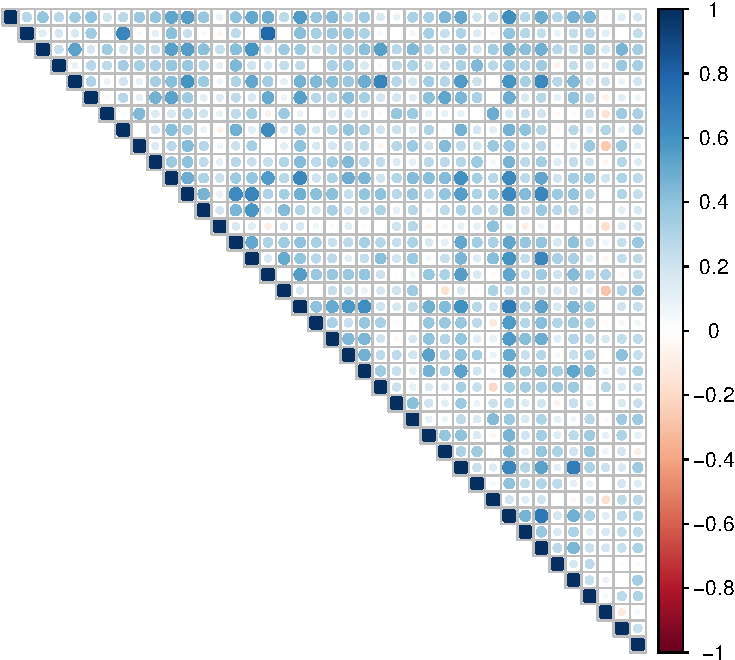
\includegraphics{TP1_files/figure-latex/correlation-1.pdf}

\end{document}
